% Appendix A

\chapter{Appendix A}
\label{AppendixA}

\section{Rejseplanen.dk screenshots}
When polite search engines, like Googlebot, access pages they first check the
rules in the server's \verb|robots.txt|. In
Figure~\ref{app:fig:rejseplanen_robots} \url{http://www.rejseplanen.dk/robots.txt} is shown;
all crawling is disabled, since \verb|Disallow| is set to \verb|/| for all agents.

\begin{figure}[htbp]
  \centering
  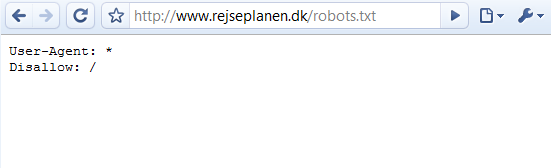
\includegraphics[width=14cm]{./Figures/rejseplanen_robots_110309}
  \rule{\textwidth}{0.005in}
  \caption{{\tt robots.txt} at \url{www.rejseplanen.dk}; [accessed 11-March-2009]}
  \label{app:fig:rejseplanen_robots}
\end{figure}

\begin{lstlisting}[caption=\url{http://www.rejseplanen.dk/},label=lst:rejseplanen.dk]
<!DOCTYPE HTML PUBLIC "-//W3C//DTD HTML 4.01 Frameset//EN">
<html>
  <head>
    <meta http-equiv="Content-Type" content="text/html; charset=ISO-8859-1">
      <title>Rejseplanen</title>
  </head>
  <frameset rows="100%">
    <frame name="rejseplanen" src="/bin/query.exe/mn">
      <noframes>
        <body>
          <a href="/bin/query.exe/mn">Videre</a> til Rejseplanen. L&#230;s mere om
          <a href="http://tog-bus.rejseplanen.dk">rejseplanl&#230;gning med kollektiv trafik</a>.
        </body>
      </noframes>
  </frameset>
</html>
\end{lstlisting}

\section{Cross-site scripting with eval}\label{sec:xss}
Imagine a site where user entered JSON data is de-serialized using the JavaScript
\verb|eval|
function\footnote{\url{https://developer.mozilla.org/en/Core_JavaScript_1.5_Reference/Global_Functions/eval}},
e.g., a site with user entered surf spots. 

Listing~\ref{lst:xss} shows how executing \verb|eval| on the user input --
hardcoded in the site in this example -- executes injected JavaScript. When the
data is evaled, the entered data is executed as if it were JavaScript. This is
used in Listing~\ref{lst:xss} to inject an extra field in the evaled data
structure. The interesting line is this:
\begin{verbatim}
{
	"name": "Ahl", attack: alert('attack'), after:""
}  
\end{verbatim}
Because the value in the \verb|attack| field is not surrounded by "", the command
\verb|alert()| is executed. We notice that this line comes from entering the
following as surf spot name:
\begin{verbatim}
  Ahl'', attack: alert('attack'), after:''
\end{verbatim}

Since it is valid JavaScript syntax, but not JSON syntax the attack is realizable
only if the response is not parsed as JSON. The attack can be tried out in action
by going to \url{http://welovewind.appspot.com/examples/xss.html}.

\begin{lstlisting}[caption=xss.html,label=lst:xss]
<!DOCTYPE html PUBLIC "-//W3C//DTD XHTML 1.0 Strict//EN"
    "http://www.w3.org/TR/xhtml1/DTD/xhtml1-strict.dtd">
<html xmlns="http://www.w3.org/1999/xhtml">
  <head>
    <meta http-equiv="content-type" content="text/html; charset=utf-8"/>
	<title>JSON eval() issues</title>
    
    <script type="text/javascript">
    //<![CDATA[
		function run(id) {
			json = document.getElementById(id).innerHTML;
			res = eval('(' + json + ')');
			return res;
		}
    //]]>
    </script>
  </head>
  <body>
  	<h1>JSON eval() issues</h1>
		<h2>Example</h2>
		<pre id="ex1">
{
	"name": "Ahl", attack: alert('attack'), after:""
}
		</pre>
		<button onclick="run('ex1');">eval it!</button>
  </body>
</html>
\end{lstlisting}